\documentclass[12pt]{article}
\usepackage{amssymb,mathrsfs, amsmath,amsfonts}
\usepackage{mathtools}
\usepackage{graphicx}
\usepackage{enumitem}
\usepackage{braket}
\graphicspath{ {./ps4-assets/}{./exercises/handwritten/ps4/ps4-assets/} }

\title{Problem Set 4 Solutions\\(published March 2024)}
\author{CSE 468}
\date{\today}

\begin{document}

\maketitle

\begin{enumerate}[font=\bfseries]
    \item Math shown below.
    \[CZ(H \otimes I) = \frac{1}{\sqrt{2}}
    \begin{pmatrix}
    1 & 0 & 1 & 0 \\
    0 & 1 & 0 & 1 \\
    1 & 0 & -1 & 0 \\
    0 & -1 & 0 & 1
    \end{pmatrix}
    \]
    No the state obtained is not entangled. Most easily verified by testing circuit with Qiskit. Analytic reasoning given below:
    \[H \otimes I = \frac{1}{\sqrt{2}}\begin{pmatrix}
    1 & 0 & 1 & 0 \\
    0 & 1 & 0 & 1 \\
    1 & 0 & -1 & 0 \\
    0 & 1 & 0 & -1
    \end{pmatrix}\]
    \[CZ(H \otimes I) = \frac{1}{\sqrt{2}}
    \begin{pmatrix}
    1 & 0 & 1 & 0 \\
    0 & 1 & 0 & 1 \\
    1 & 0 & -1 & 0 \\
    0 & -1 & 0 & 1
    \end{pmatrix}
    \]
    \[\frac{1}{\sqrt{2}}
    \begin{pmatrix}
    1 & 0 & 1 & 0 \\
    0 & 1 & 0 & 1 \\
    1 & 0 & -1 & 0 \\
    0 & -1 & 0 & 1
    \end{pmatrix}
    \begin{pmatrix}
    1 \\ 0 \\ 0 \\ 0
    \end{pmatrix}
    =
    \frac{1}{\sqrt{2}}
    \begin{pmatrix}
    1 \\ 0 \\ 1 \\ 0
    \end{pmatrix}
    \]
    \item No, the controlled Z gate cannot be written as the tensor product of two matrices. Note the controlled Z gate can be written as (from Qiskit):
    \[\begin{pmatrix}
    1 & 0 & 0 & 0 \\
    0 & 1 & 0 & 0 \\
    0 & 0 & 1 & 0 \\
    0 & 0 & 0 & -1
    \end{pmatrix}
    \]
    If the controlled Z gate could be written as the tensor product of two matrices we would have:
    \[
    \begin{pmatrix}
    a & b  \\
    c & d  \\
    \end{pmatrix}
    \otimes
    \begin{pmatrix}
    e & f  \\
    g & h  \\
    \end{pmatrix}
    =
    \begin{pmatrix}
    1 & 0 & 0 & 0 \\
    0 & 1 & 0 & 0 \\
    0 & 0 & 1 & 0 \\
    0 & 0 & 0 & -1
    \end{pmatrix}
    \]
    This gives:
    \[ae = 1, ah = 1, de = 1, dh = -1\]
    \[aedh = -1 \neq 1 = ahde\]
    \item \ %
    \begin{enumerate}
        \item \[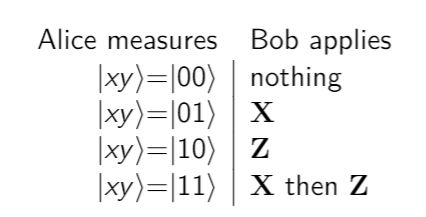
\includegraphics[scale=0.8]{teleport-action}\] 
        
        RC: The analysis below is left over from last year, and I believe the question has changed since then.  What's below is true if we know the bit is the left bit.
        
        \begin{quote}
        50\%. If Alice sends Bob a zero, he knows there's a 50\% chance that $\ket{xy} = \ket{00}$ and so he should do nothing and will obtain the correct state 50\% of the time. Similarly if Alice sends Bob a 1 he knows there's a 50\% chance that $\ket{xy} = \ket{11}$ and so he should do $\mathbf{X}$ then $\mathbf{Z}$ and will obtain the correct state 50\% of the time.
        \end{quote}
        
        RC again: If we don't know which bit is sent, then receiving a 0 eliminates $\ket{11}$ giving Bob a $1/3$ chance of getting the state right.
        
        Similarly, if a 1 is received, then that eliminates $\ket{00}$ and Bob has still a $1/3$ chance of getting the state right if he applies, say, an $\mathbf{X}$ gate.
        
        You would have gotten credit for either of the above, as you might have gotten advice based on the old question.
        
        \item If Bob knows the left qubit's value, he can tell whether he needs to apply a $\mathbf{Z}$ gate, but he will not have the appropriate magnitudes on $\ket{0}$ and $\ket{1}$ since they may be flipped.   On measurement, he thus has a 50\% chance of getting the correct result. Moreover, if he knows the left qubit he has a 50\% chance of getting the state correct.  With 0, he does nothing. With 1 he applies a $\mathbf{Z}$ gate.  And in each of those cases he has a 50\% chance of getting the state right.
        \item If Bob knows the second qubit's value he knows if his amplitudes need to be flipped or not (a X gate). If the value is 0 no flip is needed. If the value is 1 he knows he will need to apply a X gate. He does not know if he needs to apply a Z gate though.  He can thus receive the probabilistically correct result on measurement as if he has the complete state.
        \item He would want the second qubit. See (c).
    \end{enumerate}
    \item This comes from the notes, lecture 10, slide 8.  Bob must decide at random to apply ZX or not. He will obtain the correct state exactly half of the time.
    \item I follow along a similar analysis to Lecture 10 below:
    \[\ket{\psi_A\psi_B} = 
    \frac{1}{\sqrt{2}}
    \begin{pmatrix}
    0 \\ 1 \\ -1 \\ 0
    \end{pmatrix}
    ,
    \ket{\psi_x} = 
    \begin{pmatrix}
    \alpha_x \\ \beta_x
    \end{pmatrix}
    \]
    \[
    \ket{\psi_1} = \begin{pmatrix}
    \alpha_x \\ \beta_x
    \end{pmatrix}
    \otimes
    \frac{1}{\sqrt{2}}
    \begin{pmatrix}
    0 \\ 1 \\ -1 \\ 0
    \end{pmatrix}
    =
    \frac{1}{\sqrt{2}}
    \begin{pmatrix}
    0 \\ \alpha_x \\ -\alpha_x \\ 0 \\
    0 \\ \beta_x \\ -\beta_x \\ 0
    \end{pmatrix}
    \]
    \[
    \ket{\psi_2} = (CNOT \otimes I)\ket{\psi_1} = 
    \frac{1}{\sqrt{2}}
    \begin{pmatrix}
    0 \\ \alpha_x \\ -\alpha_x \\ 0 \\
    -\beta_x \\ 0 \\ 0 \\ \beta_x
    \end{pmatrix}
    \]
    8x8 matrices not included just to save space.
    \[
    \ket{\psi_3} = (H \otimes I \otimes I)\ket{\psi_2} = 
    \frac{1}{2}
    \begin{pmatrix}
    -\beta_x \\ \alpha_x \\ -\alpha_x \\ \beta_x \\
    \beta_x \\ \alpha_x \\ -\alpha_x \\ -\beta_x
    \end{pmatrix}
    \]
    \[\begin{tabular}{r|l}
\multicolumn{1}{c}{Alice measures} & \multicolumn{1}{c}{Bob's state} \\
  $\ket{xy}=\ket{00}$ & $-\beta_x\ket{0} + \alpha_x\ket{1}$  \\
  $\ket{xy}=\ket{01}$  & $-\alpha_x\ket{0} + \beta_x\ket{1}$ \\
  $\ket{xy}=\ket{10}$ & $\beta_x\ket{0} + \alpha_x\ket{1}$ \\
  $\ket{xy}=\ket{11}$ & $-\alpha_x\ket{0} - \beta_x\ket{1}$
\end{tabular}\]
    \[\begin{tabular}{r|l}
\multicolumn{1}{c}{Alice measures} & \multicolumn{1}{c}{Bob's action} \\
  $\ket{xy}=\ket{00}$ & X then Z  \\
  $\ket{xy}=\ket{01}$  & Z \\
  $\ket{xy}=\ket{10}$ & X \\
  $\ket{xy}=\ket{11}$ & Nothing
\end{tabular}\]

\item You have a 2/3 chance of measuring 0.
\end{enumerate}



\end{document}